\usetikzlibrary{trees,shadows}
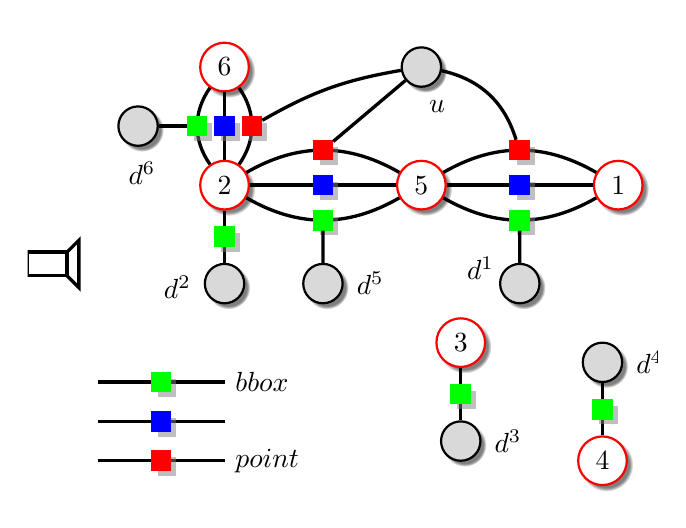
\begin{tikzpicture}[grow cyclic, line width=1.2pt,
    variablenode/.style={circle,circular drop shadow,draw=red,fill=white,thick,minimum width=0.5cm},
   bboxfactor/.style={rectangle,drop shadow,draw=green,fill=green,thick,minimum width=0.2cm},
    collfactor/.style={rectangle,drop shadow,draw=blue,fill=blue,thick,minimum width=0.2cm},
    trackfactor/.style={rectangle,drop shadow,draw=red,fill=red,thick,minimum width=0.2cm},
  obs/.style={fill=gray!30,draw=black},
  prevf/.style={draw=green!20,text=gray},
  prevobsv/.style={draw=gray!10,fill=gray!1,text=gray},
  prevv/.style={draw=red!20,text=gray}
]
  \path[use as bounding box,clip] (-2.5, -5.5) rectangle (5.5,0.5);
  \draw (-2.5,-2.65) rectangle +(0.5,0.3);
  \draw (-2.0,-2.35) -- ++(0.15, 0.15) -- ++(0, -0.6) -- (-2.0, -2.65);
\path
     (0, 0)  node [variablenode] (x6) {6}
++(0, -1.5) node [variablenode] (x2) {2}
++(2.5, 0)  node [variablenode] (x5) {5}
+ (0, 1.5)  node [variablenode,obs] (u) {}
+(.2,1.0)  node {$u$}
+ (.5, -2)   node [variablenode] (x3) {3}
+ (2.3, -3.5)   node [variablenode] (x4) {4}
+(2.5, 0)  node [variablenode] (x1) {1}
;

% Factors between nodes 6 and 2
\draw (x6) edge [bend right=35] node [bboxfactor] (f26) {} (x2);
\path (f26) +(-0.75,0) node [variablenode,obs] (d6) {} 
                        +(-.7,-.6)  node {$d^6$};
\draw (f26) edge (d6);
\draw (x6) edge [bend left=35] node [trackfactor] (ft26) {} (x2);
\draw (ft26) edge [bend left=10] (u);
\draw (x6) edge node [collfactor] {} (x2);

% Factors for node 2
\path (x2) +(0,-1.25) node [variablenode,obs] (d2) {} 
                        +(-.6,-1.3)  node {$d^2$};
\draw (x2) edge node [bboxfactor] {} (d2);

% Factors between nodes 2 and 5
\draw (x2) edge [bend right] node [bboxfactor] (f25) {} (x5);
\draw (x2) edge [bend left] node [trackfactor] (ft25) {} (x5);
\draw (x2) edge [] node [collfactor] {} (x5);
\draw (ft25) edge (u);
\path (x5) ++(-1.25,-1.25) node [variablenode,obs] (d5) {} 
                        +(.6,0)  node {$d^5$};
\draw (f25) edge (d5);

% Factors between nodes 5 and 1
\draw (x5) edge [bend right] node [bboxfactor] (f51) {} (x1);
\draw (x5) edge [bend left] node [trackfactor] (ft51) {} (x1);
\draw (x5) edge [] node [collfactor] {} (x1);
\draw (ft51) edge [bend right] (u);
\path (x1) ++(-1.25,-1.25) node [variablenode,obs] (d1) {} 
                        +(-.5,0.2)  node {$d^1$};
\draw (f51) edge (d1);

% Factors for node 3
\path (x3) ++(0,-1.25) node [variablenode,obs] (d3) {} 
                        +(.6,0)  node {$d^3$};
\draw (x3) edge node [bboxfactor] {} (d3);

% Factors for node 4
\path (x4) ++(0,1.25) node [variablenode,obs] (d4) {} 
                        +(.6,0)  node {$d^4$};
\draw (x4) edge node [bboxfactor] {} (d4);

% Legend
\path (-1.75,-4.0) node (l1s) {} (-0, -4.0) node [anchor=west] (l1e) {$\Energy{bbox}$};
\draw (l1s) edge node [bboxfactor] {} (l1e);
\path (-1.75,-4.5) node (l2s) {} (0, -4.5) node [anchor=west] (l2e) {$\EnergyCol$};
\draw (l2s) edge node [collfactor] {} (l2e);
\path (-1.75,-5.0) node (l3s) {} (0, -5.0) node [anchor=west] (l3e) {$\Energy{point}$};
\draw (l3s) edge node [trackfactor] {} (l3e);

\end{tikzpicture}
